%% sicp.tex
%% Mac Radigan
%
%% SICP documentation

\documentclass{article}[11pt]
\usepackage[]{graphics}
%\usepackage{titlesec}

%\usepackage[framed,numbered,autolinebreaks,useliterate]{mcode}
\usepackage{setspace}
\usepackage[left=1in,top=1in,right=1in,bottom=1in,nohead]{geometry}
\usepackage{graphicx,amssymb,amstext,amsmath,amsthm,caption,mathtools}
\usepackage{algorithm}
\usepackage{algorithmic}
\usepackage{amsfonts}
\usepackage{amssymb}
\bibliographystyle{IEEEtran}
%\usepackage{csvtools}
\usepackage{pdftexcmds}
%\usepackage{minted}
\usepackage{fancyvrb}
\usepackage{float}
\usepackage{csquotes}
\usepackage[skins,minted]{tcolorbox}
\usepackage{enumitem}
\usepackage{enumerate}
%\titleformat{\section}[block]{\Large\bfseries\filcenter}{}{}{}
%\newcommand\Quote[1]{\lq\textsl{#1}\rq}
%\newcommand\fr[2]{{\textstyle\frac{#1}{#2}}}
%\newcommand{\ssection}[1]{\section[#1]{\centering\normalfont\scshape #1}}
%\newcommand{\ssubsection}[1]{\subsection[#1]{\raggedright\normalfont\itshape #1}}

\usepackage{mdframed}

\usepackage{hyperref}
\hypersetup{
  colorlinks,
  citecolor=black,
  filecolor=black,
  linkcolor=black,
  urlcolor=black
}

\newcommand{\text}[1]{\\\indent\indent\indent\texttt{\footnotesize #1}\\}

\newcommand{\shellcmd}[1]{\\\indent\indent\indent\texttt{\footnotesize\# #1}\\}

\definecolor{bashbg}{rgb}{0.95,0.95,0.95}
\definecolor{schemebg}{rgb}{0.95,0.95,0.95}
\definecolor{outbg}{rgb}{0.98, 0.98, 0.82}

\newcommand{\bashlist}[1]{
 \begin{mdframed}[linecolor=black, topline=true, bottomline=true, leftline=false, rightline=false, backgroundcolor=bashbg]
 \inputminted[
   fontfamily=tt,
   fontsize=\footnotesize,
   linenos=true,
   numberblanklines=true,
   numbersep=12pt,
   numbersep=5pt,
   frame=leftline,
   breaklines=true
 ]{bash}{#1}
 \end{mdframed}
}

\newcommand{\schemelist}[1]{
 \begin{mdframed}[linecolor=black, topline=true, bottomline=true, leftline=false, rightline=false, backgroundcolor=schemebg]
 \inputminted[
   fontfamily=tt,
   fontsize=\footnotesize,
   linenos=true,
   numberblanklines=true,
   numbersep=12pt,
   numbersep=5pt,
   frame=leftline,
   breaklines=true
 ]{scheme}{#1}
 \end{mdframed}
}

\newcommand{\schemelistOLD}[1]{
 \inputminted[
   bgcolor=schemebg,
   fontfamily=tt,
   linenos=true,
   numberblanklines=true,
   numbersep=12pt,
   numbersep=5pt,
   gobble=0,
   frame=leftline,
   framesep=2mm,
   funcnamehighlighting=true,
   tabsize=4,
   obeytabs=false,
   mathescape=false
   samepage=false,
   showspaces=false,
   showtabs =false,
   texcl=false,
   baselinestretch=1.2,
   fontsize=\footnotesize,
   breaklines=true
 ]{scheme}{#1}
}

\newcommand{\outlist}[1]{
 \inputminted[
   bgcolor=outbg,
   fontfamily=tt,
   linenos=false,
   numberblanklines=false,
   numbersep=12pt,
   numbersep=5pt,
   gobble=0,
   frame=leftline,
   framesep=2mm,
   funcnamehighlighting=true,
   tabsize=4,
   obeytabs=false,
   mathescape=false
   samepage=false,
   showspaces=false,
   showtabs =false,
   texcl=false,
   baselinestretch=1.2,
   fontsize=\footnotesize,
   breaklines=true]{scheme}{#1}
}

\begin{document}

\title{Structure and Interpretation of Computer Programs (SICP) \\ worked examples}
\author{Mac Radigan}
\date{} % comment this out if you would like to include the date
%\nocite{WikiY}
\doublespacing

\maketitle

\begin{abstract}
A collection of worked examples from Gerald Sussman's book Structure and Interpretation of Computer Programs (SICP) \cite{sicp}.
\end{abstract}

\tableofcontents
%\listoffigures

%% Chapter-1.tex
%% Mac Radigan
%
%% Examples from SICP Chapter 1

    \section{Building Abstractions with Procedures}
        \subsection{The Elements of Programming}
            \subsubsection{Expressions}
Exercise 1.1. Below is a sequence of expressions. What is the result printed by the interpreter in response to each expression? Assume that the sequence is to be evaluated in the order in which it is presented.
\newline
              \schemelist{../chapter-1/sicp_ch1_e1-1.scm}
              \outlist{../output/sicp_ch1_e1-1.out}
            \subsubsection{Naming and the Environment}
Exercise 1.2. Translate the following expression into prefix form
\newline
\begin{equation}
\frac{5 + 1/2 + \left(2 - \left(3 - \left(6 + 1/5\right) \right) \right)}{3 \left( 6 - 2 \right) \left( 2 - 7 \right)}
\end{equation}
\newline
              \schemelist{../chapter-1/sicp_ch1_e1-2.scm}
              \outlist{../output/sicp_ch1_e1-2.out}
            \subsubsection{Evaluating Combinations}
Exercise 1.3. Define a procedure that takes three numbers as arguments and returns the sum of the squares of the two larger numbers.
\newline
              \schemelist{../chapter-1/sicp_ch1_e1-3.scm}
              \outlist{../output/sicp_ch1_e1-3.out}
            \subsubsection{Compound Procedures}
Exercise 1.4. Observe that our model of evaluation allows for combinations whose operators are compound expressions. Use this observation to describe the behavior of the following procedure:
\newline
\text{(define (a-plus-abs-b a b)}
\newline
\text{((if ($<$ b 0) + -) a b))}
\newline
              \schemelist{../chapter-1/sicp_ch1_e1-4.scm}
              \outlist{../output/sicp_ch1_e1-4.out}
            \subsubsection{The Substitution Model for Procedure Application}
Exercise 1.5. Ben Bitdiddle has invented a test to determine whether the interpreter he is faced with is using applicative-order evaluation or normal-order evaluation. He defines the following two procedures:
\newline
\text{(define (p) (p))}
\newline
\text{  (define (test x y)}
\newline
\text{    (if (= x 0)}
\newline
\text{    0}
\newline
\text{    y))}
\newline
Then he evaluates the expression
\newline
\text{(test 0 (p))}
\newline
What behavior will Ben observe with an interpreter that uses applicative-order evaluation? What behavior will he observe with an interpreter that uses normal-order evaluation? Explain your answer.  (Assume that the evaluation rule for the special form if is the same whether the interpreter is using normal or applicative order: The predicate expression is evaluated first, and the result determines whether to evaluate the consequent or the alternative expression.)
\newline

              % infinite loop (do not include output listing)
              \schemelist{../chapter-1/sicp_ch1_e1-5.scm}
              \outlist{../output/sicp_ch1_e1-5.out}
            \subsubsection{Conditional Expressions and Predicates}
            \subsubsection{Example: Square Roots by Newton's Method}
Exercise 1.7. The good-enough? test used in computing square roots will not be very effective for finding the square roots of very small numbers. Also, in real computers, arithmetic operations are almost always performed with limited precision. This makes our test inadequate for very large numbers. Explain these statements, with examples showing how the test fails for small and large numbers. An alternative strategy for implementing good-enough? is to watch how guess changes from one iteration to the next and to stop when the change is a very small fraction of the guess. Design a square-root procedure that uses this kind of end test. Does this work better for small and large numbers?
\newline

Newton's method:
\begin{equation}
x_{n+1} = x_{n} - \frac{f\left(x_n\right)}{f^{'}\left(x_n\right)}
\label{eq:newtons}
\end{equation}

Applied to square root:
\begin{equation}
x_{n+1} 
= x_{n} - \frac{x^2_n - \mbox{guess}}{2 x_n}
\label{eq:newtons_sqrt}
\end{equation}

              \schemelist{../chapter-1/sicp_ch1_e1-7.scm}
              \outlist{../output/sicp_ch1_e1-7.out}
            \subsubsection{Procedures as Black-Box Abstractions}
        \subsection{Procedures and the Processes They Generate}
            \subsubsection{Linear Recursion and Iteration}
Exercise 1.9: Each of the following two procedures defines a method for adding two positive integers in terms of the procedures inc, which increments its argument by 1, and dec, which decrements its argument by 1.
\newline
              \schemelist{../chapter-1/sicp_ch1_e1-9.scm}
              \outlist{../output/sicp_ch1_e1-9.out}

Exercise 1.11: A function f is defined by the rule that 

\begin{equation}
f\left(n\right) = 
\begin{cases}
n & n < 3 \\
1 f\left(n-1\right) + 2 f\left(n-2\right) + 3 f\left(n-3\right) & \mbox{ otherwise }
\end{cases}
\label{eq:ss_recursive}
\end{equation}

Write a procedure that computes f by means of a recursive process. Write a procedure that computes f by means of an iterative process.
\newline

Representing State Space Transitions
\newline

Direct Iterative Implementation
\newline

\begin{equation}
f\left(n\right) \coloneqq s_0
\label{eq:direct_def}
\end{equation}

with state transition

\begin{equation}
\stackrel{\mbox{T}}{
\left[ \begin{array}{c}
s_0 \leftarrow s_0 + 2 s_1 + 3 s_2 \\
s_1 \leftarrow s_0 \\
s_2 \leftarrow s_1 \\
\end{array} \right]
}
\label{eq:direct_trans}
\end{equation}

and initial conditions

\begin{equation}
\stackrel{\mbox{$S_0$}}{
\left[ \begin{array}{c}
s_0 \coloneqq 2 \\
s_1 \coloneqq 1 \\
s_2 \coloneqq 0 \\
\end{array} \right]
}
\label{eq:direct_init}
\end{equation}

Linear Feedback Shift Register (LFSR) representation
\newline

\begin{equation}
f\left(n,\underbar{s}\right)
\leftarrow
\begin{cases}
n^{th}_1 \underbar{s} & n = 0 \\
f\left( n-1, n^{th}_1 \leftangle \sigma_{1}(\underbar{s}), \left[ 1,2,3 \right] \rightangle \right) & \mbox{ otherwise }
\end{cases}
\label{eq:lfsr_def}
\end{equation}

\begin{equation}
\leftangle x, y \rightangle
\triangleq
\sum_{k} x_k y_k 
= x_k y^k
\label{eq:dotprod}
\end{equation}

\begin{equation}
n^{th}_k
\triangleq
x_k
\label{eq:nth}
\end{equation}

\begin{equation}
\sigma_k \left( \underbar{x} \right)
\triangleq
x_{\left( n + k \right) mod |x|} \forall n \in \underbar{x}
\label{eq:rotate}
\end{equation}

\begin{figure}[H]
\begin{center}
%\resizebox{7in}{!}{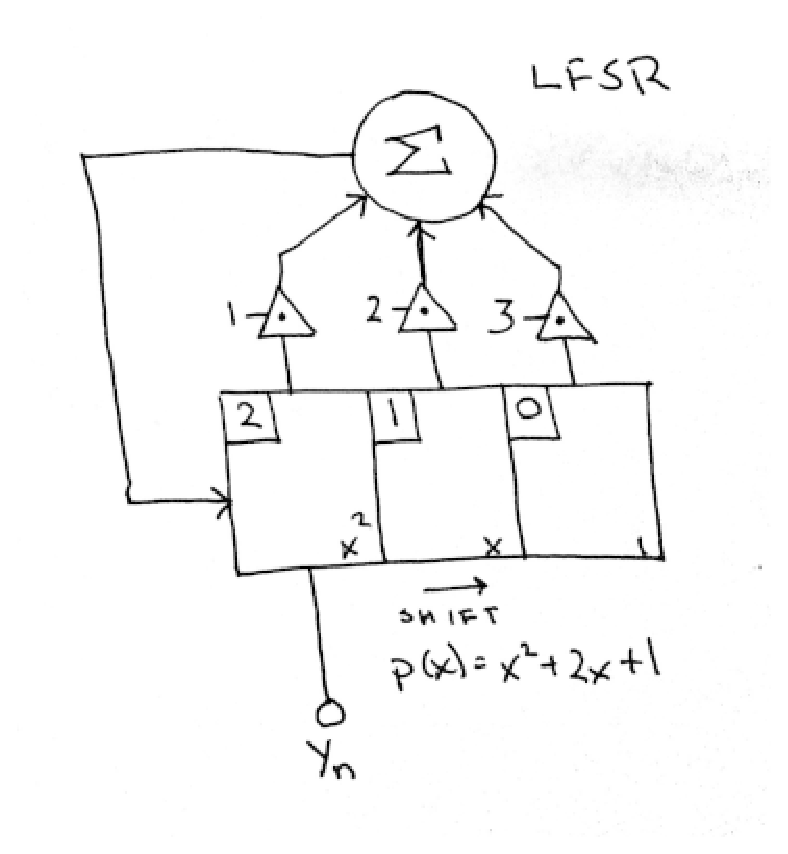
\includegraphics{./figures/lfsr-2.eps}
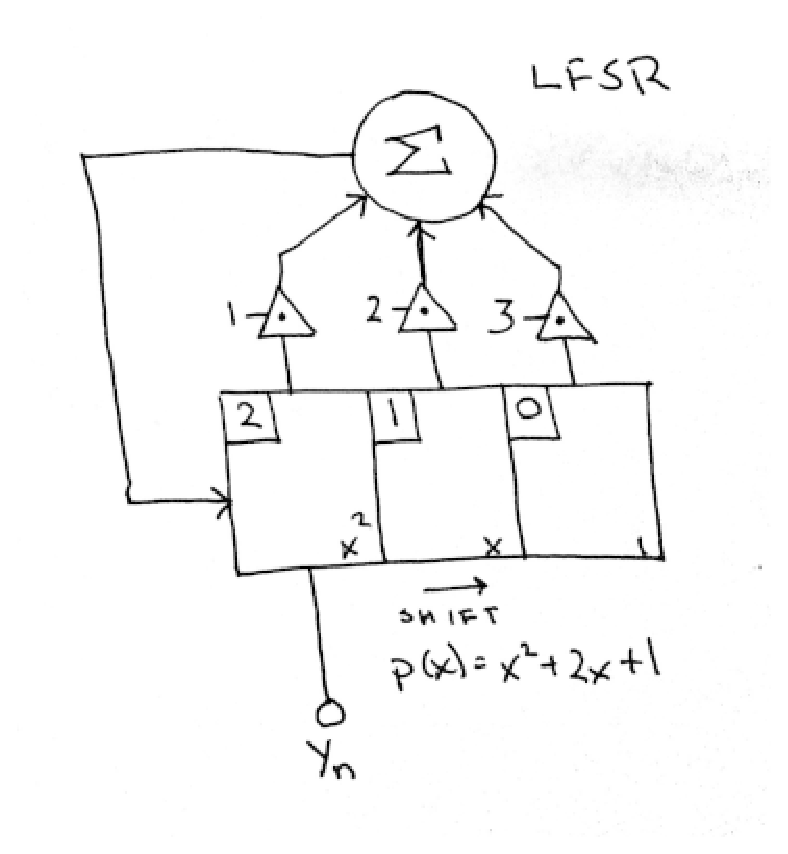
\includegraphics{./figures/lfsr-2.eps}
\end{center}
\caption{Linear Feedback Shift Register (LFSR)}
\label{fig:lfsr}
\end{figure}

State Space Representation
\newline

\begin{equation}
\mathbf{X}_k = \mathbf{F}\mathbf{X}_{k-1}
\label{eq:ss_rep}
\end{equation}

\begin{equation}
\stackrel{\mbox{$X_k$}}{
\left[ \begin{array}{c}
x^{'}_{0} \\
x^{'}_{1} \\
x^{'}_{2} \\
\end{array} \right]
}
= 
\stackrel{\mbox{$F$}}{
\left[ \begin{array}{ccc}
1 & 2 & 3 \\
1 & 0 & 0 \\
0 & 1 & 0 \\
\end{array} \right]
}
\stackrel{\mbox{$X_{k-1}$}}{
\left[ \begin{array}{c}
x_{0} \\
x_{1} \\
x_{2} \\
\end{array} \right]
}
\label{eq:ss_rep_2}
\end{equation}

where

\begin{equation}
\mathbf{X}_0 = 
\stackrel{\mbox{$X_{0}$}}{
\left[ \begin{array}{c}
2 \\
1 \\
0 \\
\end{array} \right]
}
\label{eq:ss_x0}
\end{equation}

so

\begin{equation}
\mathbf{X}_k 
= \mathbf{F}\mathbf{X}_{k-1}
= \mathbf{F} \left( \mathbf{F}\mathbf{X}_{k-2} \right)
= \mathbf{F} \left( \mathbf{F} \left( \mathbf{F}\mathbf{X}_{k-3} \right) \right)
= \cdots
= \mathbf{F}^N \mathbf{X}_0
\label{eq:ss_rep_expanded}
\end{equation}

              \schemelist{../chapter-1/sicp_ch1_e1-11.scm}
              \outlist{../output/sicp_ch1_e1-11.out}
            \subsubsection{Tree Recursion}
            \subsubsection{Orders of Growth}
            \subsubsection{Exponentiation}
Exercise 1.16:  Design a procedure that evolves an iterative exponentiation process that uses successive squaring and uses a logarithmic number of steps, as does fast-expt.  (Hint: Using the observation that $\left(b^{\frac{n}{2}}\right)^2 = \left(b^2\right)^{\frac{n}{2}}$, keep, along with the exponent n and the base b, an additional state variable a, and define the state transformation in such a way that the product a bn is unchanged from state to state. At the beginning of the process a is taken to be 1, and the answer is given by the value of a at the end of the process. In general, the technique of defining an invariant quantity that remains unchanged from state to state is a powerful way to think about the design of iterative algorithms.)

\begin{equation}
f_{benchmark}\left(x,n\right) =
\begin{cases}
1 & \mbox{ if n is zero } \\
f_{benchmark}\left(x,\frac{n}{2}\right)^{2} & \mbox{ if n is even, nonzero } \\
f_{benchmark}\left(x,n-1\right)^{2} & \mbox{ if n is odd }
\end{cases}
\label{eq:fast_expt_benchmark}
\end{equation}

may be restructured as

\begin{equation}
f\left(x,n\right) = f_{k}\left(x,n,p\right)
\label{eq:fast_expt_fast}
\end{equation}

where

\begin{equation}
f_{k}\left(x,n,p\right) =
\begin{cases}
p & \mbox{ if n is zero } \\
f_{k}\left(x,\frac{n}{2},p\right) & \mbox{ if n is even, nonzero } \\
f_{k}\left(x,n-1,p \cdot x\right) & \mbox{ if n is odd }
\end{cases}
\label{eq:fast_expt_fast_recur}
\end{equation}

              \schemelist{../chapter-1/sicp_ch1_e1-16.scm}
              \outlist{../output/sicp_ch1_e1-16.out}
            \subsubsection{Greatest Common Divisors}
            \subsubsection{Example: Testing for Primality}
        \subsection{Formulating Abstractions with Higher-Order Procedures}
            \subsubsection{Procedures as Arguments}
            \subsubsection{Constructing Procedures Using Lambda}
            \subsubsection{Procedures as General Methods}
            \subsubsection{Procedures as Returned Values}
Exercise 1.42. Let $f$ and $g$ be two one-argument functions. The composition $f$ after $g$ is defined to be the function $x \mapsto f\left(g\left(x\right)\right)$. Define a procedure compose that implements composition. For example, if $inc$ is a procedure that adds 1 to its argument, $\left(\left(compose\mbox{ }square\mbox{ }inc\right) 6\right)$

              \schemelist{../chapter-1/sicp_ch1_e1-42.scm}
              \outlist{../output/sicp_ch1_e1-42.out}

%% *EOF*

%% Chapter-1.tex
%% Mac Radigan
%
%% Examples from SICP Chapter 2

    \section{Building Abstractions with Data}
        \subsection{Introduction to Data Abstraction}
            \subsubsection{Example: Arithmetic Operations for Rational Numbers}
Exercise 2.1. Define a better version of make-rat that handles both positive and negative arguments. Make-rat should normalize the sign so that if the rational number is positive, both the numerator and denominator are positive, and if the rational number is negative, only the numerator is negative.
              \schemelist{../chapter-2/sicp_ch2_e2-1.scm}
              \outlist{../output/sicp_ch2_e2-1.out}
            \subsubsection{Abstraction Barriers}

Exercise 2.2. Consider the problem of representing line segments in a plane. Each segment is represented as a pair of points: a starting point and an ending point. Define a constructor make-segment and selectors start-segment and end-segment that define the representation of segments in terms of points. Furthermore, a point can be represented as a pair of numbers: the x coordinate and the y coordinate. Accordingly, specify a constructor make-point and selectors x-point and y-point that define this representation. Finally, using your selectors and constructors, define a procedure midpoint-segment that takes a line segment as argument and returns its midpoint (the point whose coordinates are the average of the coordinates of the endpoints).  To try your procedures, you'll need a way to print points:

              \schemelist{../chapter-2/sicp_ch2_e2-2.scm}
              \outlist{../output/sicp_ch2_e2-2.out}

Exercise 2.3. Implement a representation for rectangles in a plane. (Hint: You may want to make use of exercise 2.2.) In terms of your constructors and selectors, create procedures that compute the perimeter and the area of a given rectangle. Now implement a different representation for rectangles.  Can you design your system with suitable abstraction barriers, so that the same perimeter and area procedures will work using either representation?

              \schemelist{../chapter-2/sicp_ch2_e2-3.scm}
              \outlist{../output/sicp_ch2_e2-3.out}
            \subsubsection{What Is Meant by Data?}
            \subsubsection{Extended Exercise: Interval Arithmetic}
        \subsection{Hierarchical Data and the Closure Property}
Exercise 2.17.  Define a procedure last-pair that returns the list that contains only the last element of a given (nonempty) list:
              \schemelist{../chapter-2/sicp_ch2_e2-17.scm}
              \outlist{../output/sicp_ch2_e2-17.out}
Exercise 2.18.  Define a procedure reverse that takes a list as argument and returns a list of the same elements in reverse order:
              \schemelist{../chapter-2/sicp_ch2_e2-18.scm}
              \outlist{../output/sicp_ch2_e2-18.out}
            \subsubsection{Representing Sequences}
            \subsubsection{Hierarchical Structures}
            \subsubsection{Sequences as Conventional Interfaces}
            \subsubsection{Example: A Picture Language}
Exercise 2.44.  Define the procedure up-split used by corner-split.  It is similar to right-split, except that it switches the roles of below and beside.
              \schemelist{../chapter-2/sicp_ch2_e2-44.scm}
              \outlist{../output/sicp_ch2_e2-44.out}

\begin{figure}[H]
\begin{center}
%\resizebox{7in}{!}{\includegraphics{../figures/sicp_ch2_e2-44.png}}
\includegraphics{../figures/sicp_ch2_e2-44.png}
\end{center}
\caption{Up Split 2}
\label{fig:up_split_2}
\end{figure}

Exercise 2.45.  Right-split and up-split can be expressed as instances of a general splitting operation. Define a procedure split with the property that evaluating
\begin{verbatim}
  (define right-split (split beside below))
  (define up-split (split below beside))
\end{verbatim}
produces procedures right-split and up-split with the same behaviors as the ones already defined.
              \schemelist{../chapter-2/sicp_ch2_e2-45.scm}
              \outlist{../output/sicp_ch2_e2-45.out}

\begin{figure}[H]
\begin{center}
%\resizebox{7in}{!}{\includegraphics{../figures/sicp_ch2_e2-45_right.png}}
\includegraphics{../figures/sicp_ch2_e2-45_right.png}
\end{center}
\caption{Right Split 2}
\label{fig:right_split_2}
\end{figure}

\begin{figure}[H]
\begin{center}
%\resizebox{7in}{!}{\includegraphics{../figures/sicp_ch2_e2-45_up.png}}
\includegraphics{../figures/sicp_ch2_e2-45_up.png}
\end{center}
\caption{Up Split 2}
\label{fig:up_split_2}
\end{figure}

Exercise 2.46.  A two-dimensional vector v running from the origin to a point can be represented as a pair consisting of an x-coordinate and a y-coordinate. Implement a data abstraction for vectors by giving a constructor make-vect and corresponding selectors xcor-vect and ycor-vect. In terms of your selectors and constructor, implement procedures add-vect, sub-vect, and scale-vect that perform the operations vector addition, vector subtraction, and multiplying a vector by a scalar:
              \schemelist{../chapter-2/sicp_ch2_e2-46.scm}
              \outlist{../output/sicp_ch2_e2-46.out}

        \subsection{Symbolic Data}
            \subsubsection{Quotation}

Exercise 2.54. Two lists are said to be equal? if they contain equal 
elements arranged in the same order. For example,
\newline

(equal? '(this is a list) '(this is a list))
\newline

is true, but
\newline

(equal? '(this is a list) '(this (is a) list))
\newline

is false. To be more precise, we can define equal? recursively in terms of 
\newline

the basic eq? equality of symbols by saying that a and b are equal? if 
they are both symbols and the symbols are eq?, or if they are both lists 
such that (car a) is equal? to (car b) and (cdr a) is equal? to (cdr b). 
Using this idea, implement equal? as a procedure. 
\newline

Comparing to structures using $equals?$:
\newline

\begin{equation}
\left(equals?\mbox{ a b}\right) = 
f\left(a,b\right) = 
\begin{cases}
\bot                                                  & \mbox{if } S\left(a\right) \oplus S\left(b\right) \\
a \stackrel{?}{=} b                                   & \mbox{if } S\left(a\right) \wedge S\left(b\right) \\
f\left(a_A,b_A\right) \lwedge f\left(a_D,b_D\right)   & \mbox{if } L\left(a\right) \wedge L\left(b\right)
\end{cases}
\label{eq:def_equals}
\end{equation}
\newline

\text{where}
\newline

\begin{equation}
L\left(a\right) \wedge L\left(b\right)
\Longrightarrow
\lnot \left( S\left(a\right) \wedge S\left(b\right) \right)
\end{cases}
\label{eq:def_equals_membership}
\end{equation}


To show that all cases have been exhausted (\ref{eq:def_equals_table}):
\newline

\begin{equation}
\begin{array}{cc|ccc}
S\left(a\right) & 
S\left(b\right) & 
S\left(a\right) \wedge S\left(b\right) & 
S\left(a\right) \oplus S\left(b\right) & 
\lnot \left( S\left(a\right) \wedge S\left(b\right) \right)
\\
\hline
F & F & F                   & F                       & \textcolor{blue}{T} \\
F & T & F                   &     \textcolor{blue}{T} & F                   \\
T & F & F                   &     \textcolor{blue}{T} & F                   \\
T & T & \textcolor{blue}{T} & F                       & F                   \\
\end{array}
\label{eq:def_equals_table}
\end{equation}

At this point, the recursive form is functional, but it is not expressed in tail-recursive form, and as such is not subject to tail-call optimization.  The following is a conversion to tail-recursive form:
\newline
\begin{equation}

\begin{equation}
\left(equals?\mbox{ a b}\right) = 
f\left(a,b\right) = f_k\left(a,b,\top\right)
\label{eq:def_equals_tco}
\end{equation}
\newline

\begin{equation}
f_k\left(a,b,p\right) = 
\begin{cases}
\bot                                                & \mbox{if } S\left(a\right) \oplus S\left(b\right) \\
p \wedge \left( a \stackrel{?}{=} b \right)         & \mbox{if } S\left(a\right) \wedge S\left(b\right) \\
f_k\left(a_D,b_D, f_k\left(a_A,b_A,p\right)\right)  & \mbox{otherwise}
\end{cases}
\label{eq:def_equals_tco_iter}
\end{equation}
\newline

              \schemelist{../chapter-2/sicp_ch2_e2-54.scm}
              \outlist{../output/sicp_ch2_e2-54.out}
Exercise 2.55. Eva Lu Ator types to the interpreter the expression (car 'abracadabra)
\newline
To her surprise, the interpreter prints back quote. Explain.
              \schemelist{../chapter-2/sicp_ch2_e2-55.scm}
              \outlist{../output/sicp_ch2_e2-55.out}
            \subsubsection{Example: Symbolic Differentiation}
Exercise 2.56.  Show how to extend the basic differentiator to handle more kinds of expressions. For instance, implement the differentiation rule
\begin{equation}
\frac{\partial d \left( u^n \right)}{\partial u}
= n u^{-1} \frac{\partial u}{\partial x}
\label{eq:deriv_exp}
\end{equation}
\newline
              \schemelist{../chapter-2/sicp_ch2_e2-56.scm}
              \outlist{../output/sicp_ch2_e2-56.out}
            \subsubsection{Example: Representing Sets}
            \subsubsection{Example: Huffman Encoding Trees}
        \subsection{Multiple Representations for Abstract Data}
            \subsubsection{Representations for Complex Numbers}
            \subsubsection{Tagged data}
            \subsubsection{Data-Directed Programming and Additivity}
        \subsection{Systems with Generic Operations}
            \subsubsection{Generic Arithmetic Operations}
            \subsubsection{Combining Data of Different Types}
            \subsubsection{Example: Symbolic Algebra}

%% *EOF*

%% Chapter-1.tex
%% Mac Radigan
%
%% Examples from SICP Chapter 3

    \section{Modularity, Objects, and State}
        \subsection{Assignment and Local State}
            \subsubsection{Local State Variables}
            \subsubsection{The Benefits of Introducing Assignment}
            \subsubsection{The Costs of Introducing Assignment}
        \subsection{The Environment Model of Evaluation}
            \subsubsection{The Rules for Evaluation}
            \subsubsection{Applying Simple Procedures}
            \subsubsection{Frames as the Repository of Local State}
            \subsubsection{Internal Definitions}
        \subsection{Modeling with Mutable Data}
            \subsubsection{Mutable List Structure}
            \subsubsection{Representing Queues}
            \subsubsection{Representing Tables}
            \subsubsection{A Simulator for Digital Circuits}
            \subsubsection{Propagation of Constraints}
        \subsection{Concurrency: Time Is of the Essence}
            \subsubsection{The Nature of Time in Concurrent Systems}
            \subsubsection{Mechanisms for Controlling Concurrency}
        \subsection{Streams}
            \subsubsection{Streams Are Delayed Lists}
              \schemelist{../chapter-3/sicp_ch3_e3-50.scm}
            \subsubsection{Infinite Streams}
            \subsubsection{Exploiting the Stream Paradigm}
            \subsubsection{Streams and Delayed Evaluation}
            \subsubsection{Modularity of Functional Programs and Modularity of Objects}

%% *EOF*

%% Chapter-1.tex
%% Mac Radigan
%
%% Examples from SICP Chapter 4

    \section{Metalinguistic Abstraction}
        \schemelist{../chapter-4/run-query.scm}
        \subsection{The Metacircular Evaluator}
            \subsubsection{The Core of the Evaluator}
            \subsubsection{Representing Expressions}
            \subsubsection{Evaluator Data Structures}
            \subsubsection{Running the Evaluator as a Program}
            \subsubsection{Data as Programs}
            \subsubsection{Internal Definitions}
            \subsubsection{Separating Syntactic Analysis from Execution}
        \subsection{Variations on a Scheme -- Lazy Evaluation}
            \subsubsection{Normal Order and Applicative Order}
            \subsubsection{An Interpreter with Lazy Evaluation}
            \subsubsection{Streams as Lazy Lists}
        \subsection{Variations on a Scheme -- Nondeterministic Computing}
            \subsubsection{Amb and Search}
            \subsubsection{Examples of Nondeterministic Programs}
            \subsubsection{Implementing the Amb Evaluator}
        \subsection{Logic Programming}
An excellent discussion of logic programming can be found in chapter 19 of Paul Graham's \emph{On Lisp} \cite{Graham}.
            \subsubsection{Deductive Information Retrieval}
Exercise 4.55.  Give simple queries that retrieve the following information from the data base:
\begin{enumerate}[(a)]
\item all people supervised by Ben Bitdiddle;
\item the names and jobs of all people in the accounting division;
\item the names and addresses of all people who live in Slumerville.
\end{enumerate}
              \schemelist{../chapter-4/sicp_ch4_e4-55.scm}
              \outlist{../output/sicp_ch4_e4-55.out}
Exercise 4.56.  Formulate compound queries that retrieve the following information:
\begin{enumerate}[(a)]
\item the names of all people who are supervised by Ben Bitdiddle, together with their addresses;
\item all people whose salary is less than Ben Bitdiddle's, together with their salary and Ben Bitdiddle's salary;
\item all people who are supervised by someone who is not in the computer division, together with the supervisor's name and job.
\end{enumerate}
              \schemelist{../chapter-4/sicp_ch4_e4-56.scm}
              \outlist{../output/sicp_ch4_e4-56.out}
            \subsubsection{How the Query System Works}

\begin{algorithm}
\caption{Driver Loop}
\label{alg:driver_loop}
\Procedure{Driver}{}
  \State \Comment{Main Query REPL}
  \State $\mbox{let  } q \leftarrow \mathbf{READ}$
  \If{ $\mbox{Assertion-To-Be-Added?  } q$ }
    \State $\mbox{Add-Rule-Or-Assertion!  } \leftarrow q$
  \Else
    \State $\mbox{Display-Stream } \mbox{Stream-Map } \mbox{  } \texttt{\char`\\}$
    \State $\lambda f . \mathbf{Instantiate}(q\mbox{,}f\mbox{,} \lambda v f . \mbox{ccm}(v)) \mbox{  } \texttt{\char`\\}$
    \State $\mathbf{qeval}(q\mbox{,the-stream})$
  \EndIf
\EndProcedure
\end{algorithm}
\newline
\schemelist{./ch4_driver.scm}
\newline

\begin{algorithm}
\caption{Instantiate}
\label{alg:connected}
\Function{Instantiate}{\mathbb{e}:Expression, \mathbb{f}:Frame \mathbb{h}:Handler}
  \State \Comment{Instantiate Binding Variables}
  \Function{Copy}{\mathbb{e}:Expression}
    \If{var? \mathbf{e}}
      \State $\mbox{let } \mbox{b := f}\left[ e \right]$
      \If{\mathbf{b}}
        \State $Copy(b_D)$
        \State \Comment{Contract Question Mark (ccm) with Handler h}
        \State $ccm(e)$
      \EndIf
    \EndIf
    \If{pair? \mathbf{e}}
      \State $\left[ Copy(e_A) \mbox{ } Copy(e_D) \right]$
    \EndIf
    \If{Else:}
      \State $Copy(e)$
    \EndIf
  \EndFunction
  \State $Copy(e)$
\EndFunction
\end{algorithm}
\newline
\schemelist{./ch4_instantiate.scm}
\newline

\begin{algorithm}
\caption{Qeval}
\label{alg:qeval}
\Function{Qeval}{\mathbb{q}:Query, \mathbb{s}:FrameStream}
  \State \Comment{Evaluate Query}
  \State $\mbox{let } \mbox{f := } \mathbf{getProc}(q)$
  \If{f}
    \State $\mathbf{f}(q_D,s)$
  \Else
    \State $\mathbf{SimpleQuery}(q_D,s)$
  \EndIf
\EndFunction
\end{algorithm}
\newline
\schemelist{./ch4_qeval.scm}
\newline

\begin{algorithm}
\caption{SimpleQuery}
\label{alg:simplequery}
\Function{SimpleQuery}{\mathbb{p}:QueryPattern, \mathbb{s}:FrameStream}
  \State \Comment{Evaluate Simple Query}
  \State $\mbox{stream-flatmap } \texttt{\char`\\}$
  \State $\mbox{   } \lambda f . \mathbf{StreamAppendDelayed}( \mbox{ } \mathbf{FindAssertions}(p,f) \mbox{ , } \mathbf{Delay}(\mathbf{ApplyRules}(p,s)) \mbox{ } ) \mbox{ } \texttt{\char`\\}$
  \State $\mbox{   } fs$
\EndFunction
\end{algorithm}
\newline
\schemelist{./ch4_simple_query.scm}
\newline

            \subsubsection{Is Logic Programming Mathematical Logic?}
            \subsubsection{Implementing the Query System}

%% *EOF*

%% Chapter-1.tex
%% Mac Radigan
%
%% Examples from SICP Chapter 5

    \section{Computing with Register Machines}
        \subsection{Designing Register Machines}
            \subsubsection{A Language for Describing Register Machines}
            \subsubsection{Abstraction in Machine Design}
            \subsubsection{Subroutines}
            \subsubsection{Using a Stack to Implement Recursion}
            \subsubsection{Instruction Summary}
        \subsection{A Register-Machine Simulator}
            \subsubsection{The Machine Model}
            \subsubsection{The Assembler}
            \subsubsection{Generating Execution Procedures for Instructions}
            \subsubsection{Monitoring Machine Performance}
        \subsection{Storage Allocation and Garbage Collection}
            \subsubsection{Memory as Vectors}
            \subsubsection{Maintaining the Illusion of Infinite Memory}
        \subsection{The Explicit-Control Evaluator}
            \subsubsection{The Core of the Explicit-Control Evaluator}
            \subsubsection{Sequence Evaluation and Tail Recursion}
            \subsubsection{Conditionals, Assignments, and Definitions}
            \subsubsection{Running the Evaluator}
        \subsection{Compilation}
            \subsubsection{Structure of the Compiler}
            \subsubsection{Compiling Expressions}
            \subsubsection{Compiling Combinations}
            \subsubsection{Combining Instruction Sequences}
            \subsubsection{An Example of Compiled Code}
            \subsubsection{Lexical Addressing}
            \subsubsection{Interfacing Compiled Code to the Evaluator}

%% *EOF*


%% Appendix-Library.tex
%% Mac Radigan

\section{Appendix A: Modules}
\label{sec:appendix_a}
\subsection{util.scm}
\schemelist{../library/util.scm}

%% *EOF*

%% Appendix-Library.tex
%% Mac Radigan

\section{Appendix B: Installation Notes}
\label{sec:appendix_b}
\subsection{Chicken Scheme}
\bashlist{../install/apt-install.sh}
\bashlist{../install/yum-install.sh}
\bashlist{../install/brew-install.sh}
\bashlist{../install/chicken-install.sh}

%% *EOF*

%% Appendix-Notation.tex
%% Mac Radigan

\section{Appendix C: Notation}
\label{sec:appendix_notation}

\subsection{Membership}

\begin{equation}
S\left(x\right) \triangleq x \in \mbox{SYMBOL}
\end{cases}
\label{eq:def_equals_symbol}
\end{equation}

\begin{equation}
L\left(x\right) \triangleq x \in \mbox{LIST}
\end{cases}
\label{eq:def_equals_list}
\end{equation}

\subsection{Symbols}

\begin{equation}
\top \triangleq \mbox{\#t}
\end{cases}
\label{eq:def_equals_true}
\end{equation}

\begin{equation}
\bot \triangleq \mbox{\#f}
\end{cases}
\label{eq:def_equals_false}
\end{equation}

\subsection{Access}

\begin{equation}
x_A \triangleq \left(\mbox{car x}\right)
\end{cases}
\label{eq:def_equals_car}
\end{equation}

\begin{equation}
x_D \triangleq \left(\mbox{cdr x}\right)
\end{cases}
\label{eq:def_equals_cdr}
\end{equation}

\subsection{Equality}

\begin{equation}
x \stackrel{?}{=} y \triangleq \left(\mbox{eq? x y}\right)
\end{cases}
\label{eq:def_equals_eq}
\end{equation}

\subsection{Logic}

\begin{equation}
\lnot x \triangleq \left(\mbox{not x}\right)
\end{cases}
\label{eq:def_equals_not}
\end{equation}

\begin{equation}
x \wedge y \triangleq \left(\mbox{and x y}\right)
\end{cases}
\label{eq:def_equals_and}
\end{equation}

\begin{equation}
x \lor y \triangleq \left(\mbox{or x y}\right)
\end{cases}
\label{eq:def_equals_or}
\end{equation}

\begin{equation}
x \oplus y \triangleq 
\left(\lnot x \lwedge y\right)
\lor
\left(x \lwedge \lnot y\right)
\end{cases}
\label{eq:def_equals_xor}
\end{equation}

%% *EOF*

%% Appendix-Notes.tex
%% Mac Radigan

\section{Appendix D: Y-Combinator}
\label{sec:appendix_ycombinator}
\subsection{Introduction}
     Description of the Y Combinator based on Mike Mvanier's blog post \cite{Mvanier}.
     see http://mvanier.livejournal.com/2897.html

% \begin{displayquote}
% Tiger got to hunt, bird got to fly;
% \newline
% Man got to sit and wonder 'why, why, why?'
% \newline
% Tiger got to sleep, bird got to land;
% \newline
% Man got to tell himself he understand.
% \newline
% -Kurt Vonnegut, Cat's Cradle
% \end{displayquote}
% 
% \newline
% \newline
% 
% \begin{displayquote}
% Tiger got to hunt,
% \newline
% Bird got to fly;
% \newline
% Lisper got to sit and wonder, (Y (Y Y))?
% \newline
% \newline
% Tiger got to sleep,
% \newline
% Bird got to land;
% \newline
% Lisper got to tell himself he understand.
% \newline
% - Kurt Vonnegut, modified by Darius Bacon
% \end{displayquote}

      \subsection{Cannonical Expression}

        Curry's Y Combinator \cite{WikiY} is defined as:

        \begin{equation}
        \mathbf{Y} = 
        \lambda f . 
        \left( \lambda x . f \left( x x \right) \right)
        \left( \lambda x . f \left( x x \right) \right)
        \label{eq:y_combinator}
        \end{equation}

        When applied to a function $g$, the expansion follows \cite{WikiY}

        \begin{equation}
        \begin{aligned}
        \mathbf{Y}g 
        & = \left( \lambda f .  \left( \lambda x . f \left( x x \right) \right) \left( \lambda x . f \left( x x \right) \right) \right) g \\
        & = \left( \lambda x . g \left( x x \right) \right) \left( \lambda x . g \left( x x \right) \right) \\
        & = g \left( \left( \lambda x . g \left( x x \right) \right) \left( \lambda x . g \left( x x \right) \right) \right) \\
        & = g \left( \mathbf{Y} g \right)
        \end{aligned}
        \label{eq:y_combinator_expanded}
        \end{equation}

    \subsection{Connonical Form in Scheme}
      Direct implementation of the above expression for the Y Combinator will not terminate during applicative order \cite{Mvanier}.
      \subsubsection{Strict Scheme (Chicken)}
        Chicken scheme is a strict scheme, and evaluates in applicative order.
        \schemelist{../appendices-y/src-chicken/y-combinator.scm}
      \subsubsection{Using Lazy Evaluation (Racket \#lang lazy)}
        This will work in a lazy language, as shown using the lazy extension in Racket.
        \schemelist{../appendices-y/src-racket/y-combinator.rkt-lazy}
        \outlist{../output/y-combinator-rkt-lazy.out}


  \subsection{Normal Order Y Combinator}
    The Normal Order Y Combinator will not terminate during applicative order \cite{Mvanier}.
    \subsubsection{Strict Scheme (Chicken)}
      \schemelist{../appendices-y/src-chicken/y-combinator-normal.scm}
    \subsubsection{Using Strict Evaluation (Racket)}
      \schemelist{../appendices-y/src-racket/y-combinator-normal.rkt-lazy}
    \subsubsection{Using Lazy Evaluation (Racket \#lang lazy)}
      However, it will work under lazy evaluation.
      \schemelist{../appendices-y/src-racket/y-combinator-normal.rkt-lazy}
      \outlist{../output/y-combinator-normal-rkt-lazy.out}

    \subsection{Strict (Applicative-Order) Y Combinator}
      The Strict (Applicative-Order) Y Combinator can be used with both applicative order and lazy evaluation \cite{Mvanier}.
      \subsubsection{Strict Scheme (Chicken)}
        \schemelist{../appendices-y/src-chicken/y-combinator-strict.scm}
        \outlist{../output/y-combinator-strict-scm.out}
      \subsubsection{Using Strict Evaluation (Racket)}
        \schemelist{../appendices-y/src-racket/y-combinator-strict.rkt}
        \outlist{../output/y-combinator-strict-rkt.out}
      \subsubsection{Using Lazy Evaluation (Racket \#lang lazy)}
        \schemelist{../appendices-y/src-racket/y-combinator-strict.rkt-lazy}
        \outlist{../output/y-combinator-strict-rkt-lazy.out}

%% *EOF*

%%% Appendix-Notes.tex
%% Mac Radigan

\section{Appendix D: Notes}
\label{sec:appendix_notes}
\subsection{Y-Combiner}

% \begin{displayquote}
% Tiger got to hunt, bird got to fly;
% \newline
% Man got to sit and wonder 'why, why, why?'
% \newline
% Tiger got to sleep, bird got to land;
% \newline
% Man got to tell himself he understand.
% \newline
% -Kurt Vonnegut, Cat's Cradle
% \end{displayquote}
% 
% \newline
% \newline
% 
% \begin{displayquote}
% Tiger got to hunt,
% \newline
% Bird got to fly;
% \newline
% Lisper got to sit and wonder, (Y (Y Y))?
% \newline
% \newline
% Tiger got to sleep,
% \newline
% Bird got to land;
% \newline
% Lisper got to tell himself he understand.
% \newline
% - Kurt Vonnegut, modified by Darius Bacon
% \end{displayquote}

Curry's Y-Combiner \cite{WikiY} is defined as:

\begin{equation}
\mathbf{Y} = 
\lambda f . 
\left( \lambda x . f \left( x x \right) \right)
\left( \lambda x . f \left( x x \right) \right)
\label{eq:y_combiner}
\end{equation}

When applied to a function $g$, the expansion follows \cite{WikiY}

\begin{equation}
\begin{aligned}
\mathbf{Y}g 
& = \left( \lambda f .  \left( \lambda x . f \left( x x \right) \right) \left( \lambda x . f \left( x x \right) \right) \right) g \\
& = \left( \lambda x . g \left( x x \right) \right) \left( \lambda x . g \left( x x \right) \\
& = g \left( \left( \lambda x . g \left( x x \right) \right) \left( \lambda x . g \left( x x \right) \right) \\
& = g \left( \mathbf{Y} g \right)
\end{aligned}
\label{eq:y_combiner}
\end{equation}



%% *EOF*


\nocite{*}
\bibliography{IEEEabrv,bibliography}

\end{document}

%% %EOF*
